\documentclass[accentcolor=tud9d,colorbacktitle,inverttitle,landscape,german,presentation,t]{tudbeamer}
\usepackage{ngerman}
\usepackage[T1]{fontenc}
\usepackage[latin1]{inputenc}
\usepackage{helvet}
\usepackage{graphicx}
\usepackage{picins}


\begin{document}

	% Titel
	\title{Instant Message Whispering via Covert Channels}
	\subtitle{Simon Bunten, Gruppe 35 }
	
 	% Fu�zeile
	\author{J.S. Bunten, S. Kadel, M.S. Oehler, A.S. St�hlmeyer}
	\date{\today}
	\logo{
\includegraphics{../Bilder/tklogo.jpg}}

\begin{titleframe}
	\begin{figure}
	\centering
	
\includegraphics[scale=.55]{../Bilder/InstantMessenger.jpg}
	\end{figure}
\end{titleframe}

\begin{frame}
\frametitle{Einf�hrung}
	
	\begin{minipage}{.55\linewidth}
		Verstecktes Instant Messaging
		\begin{itemize}
			\item Unentdecktes Senden von Nachrichten
			\item Umgehen von Sicherheitsvorkehrungen wie Firewalls
		\end{itemize}	
	\end{minipage}
	\hfill
	\begin{minipage}{.4\linewidth}
	{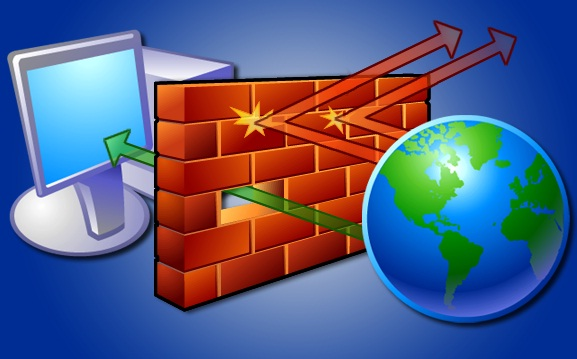
\includegraphics[scale=.3]{../Bilder/Firewall.jpg}}
	\end{minipage}
	
	\begin{description}
		\item {}
		\item{}
		\item[Kryptographie] <2>Verschl�sselt die Daten, Kanal bleibt sichtbar
		\item[Covert Channels]<2> Versteckt den Kanal
	\end{description}
	
\end{frame}

\begin{frame}
\frametitle{Covert Channel im TCP Header}
		\begin{figure}
			\centering
			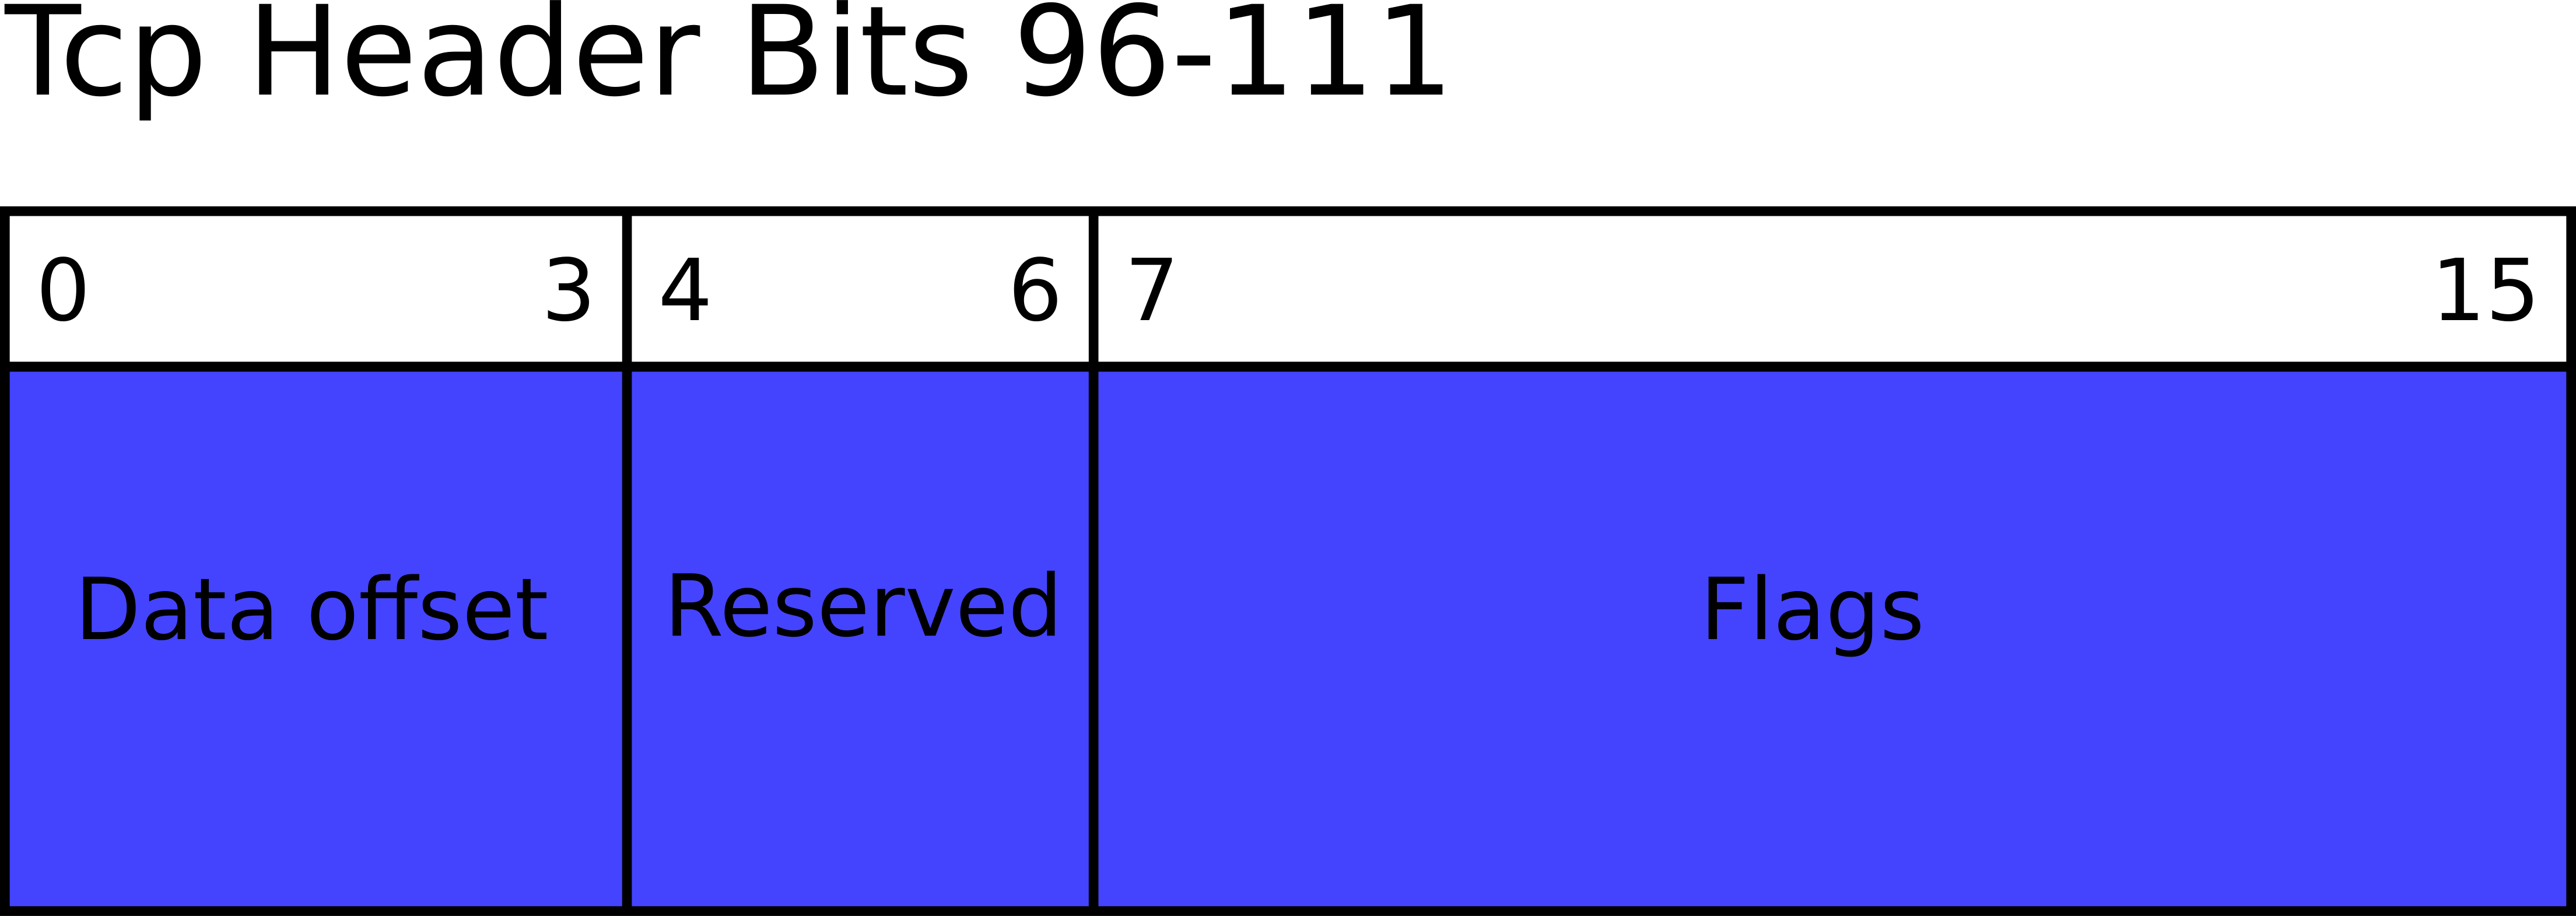
\includegraphics[scale=.5]{../Bilder/tcpHeader.png}
		\end{figure}
\end{frame}

\begin{frame}
\frametitle{Covert Channel im Inter Packet Delay}
		\begin{figure}
			\centering
			
\includegraphics[scale=.3]{../Bilder/sos.png}
		\end{figure}
\end{frame}

\begin{frame}
\frametitle{Covert Channel im Inter Packet Delay}
		\begin{figure}
			\centering
			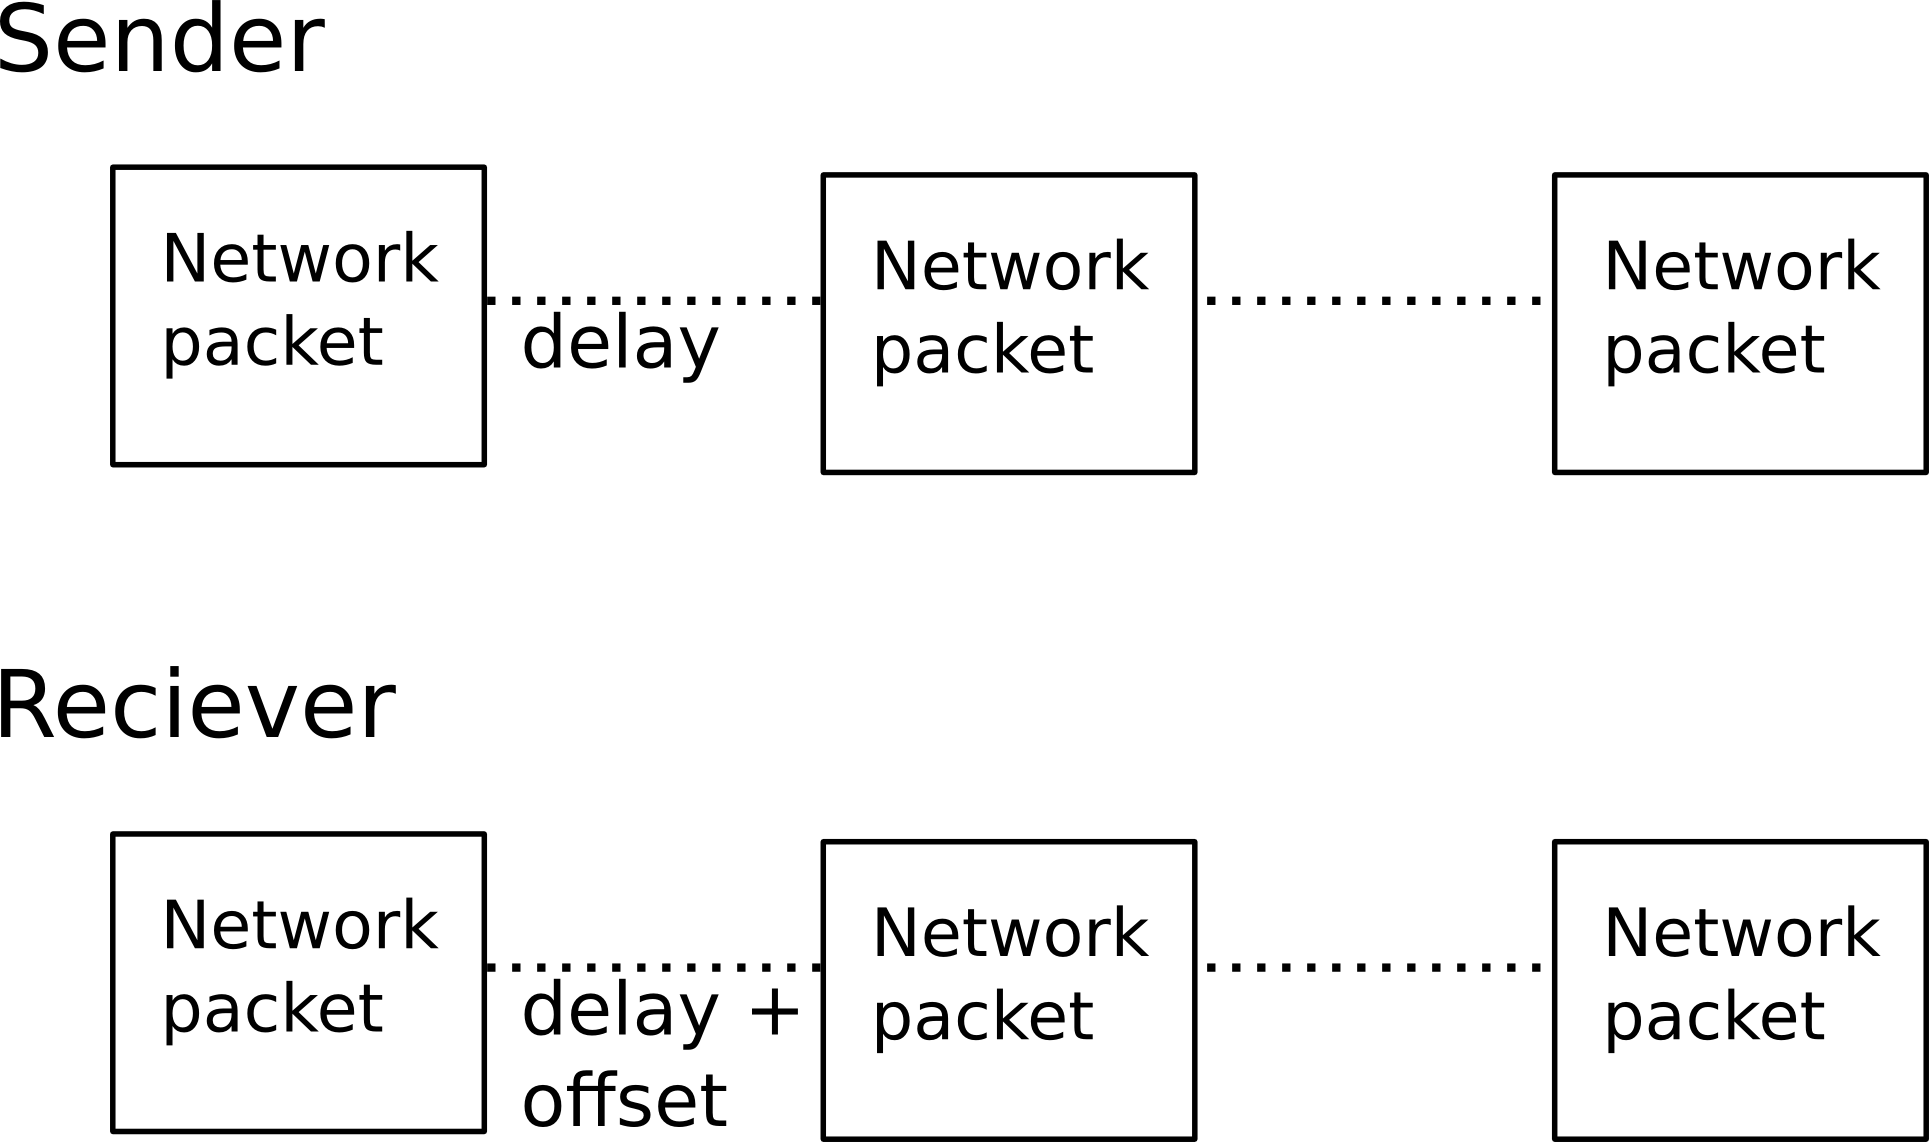
\includegraphics[scale=.5]{../Bilder/timingChannel.png}
		\end{figure}
\end{frame}

\begin{frame}

	\frametitle{Projektbeschreibung}
	Programmieren einer Bibliothek f�r Covert Channels
	\begin{itemize}
		\item <2>�ffnet und verwendet Covert Channels
		\item <2>Hilft Nutzern bei der Erstellung eigener Covert Channels
		\item <2>Ver�ffentlichung als Open Source
	\end{itemize}
	\begin{center}
		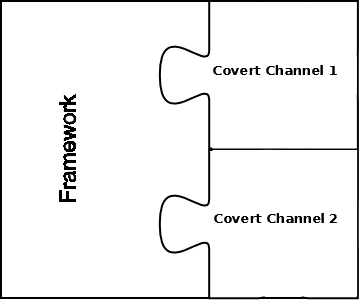
\includegraphics[scale=0.25]{../Bilder/framework-puzzle.png}
	\end{center}

\end{frame}

\begin{frame}
	\frametitle{Top-Level Design}
		\begin{figure}
			\centering
			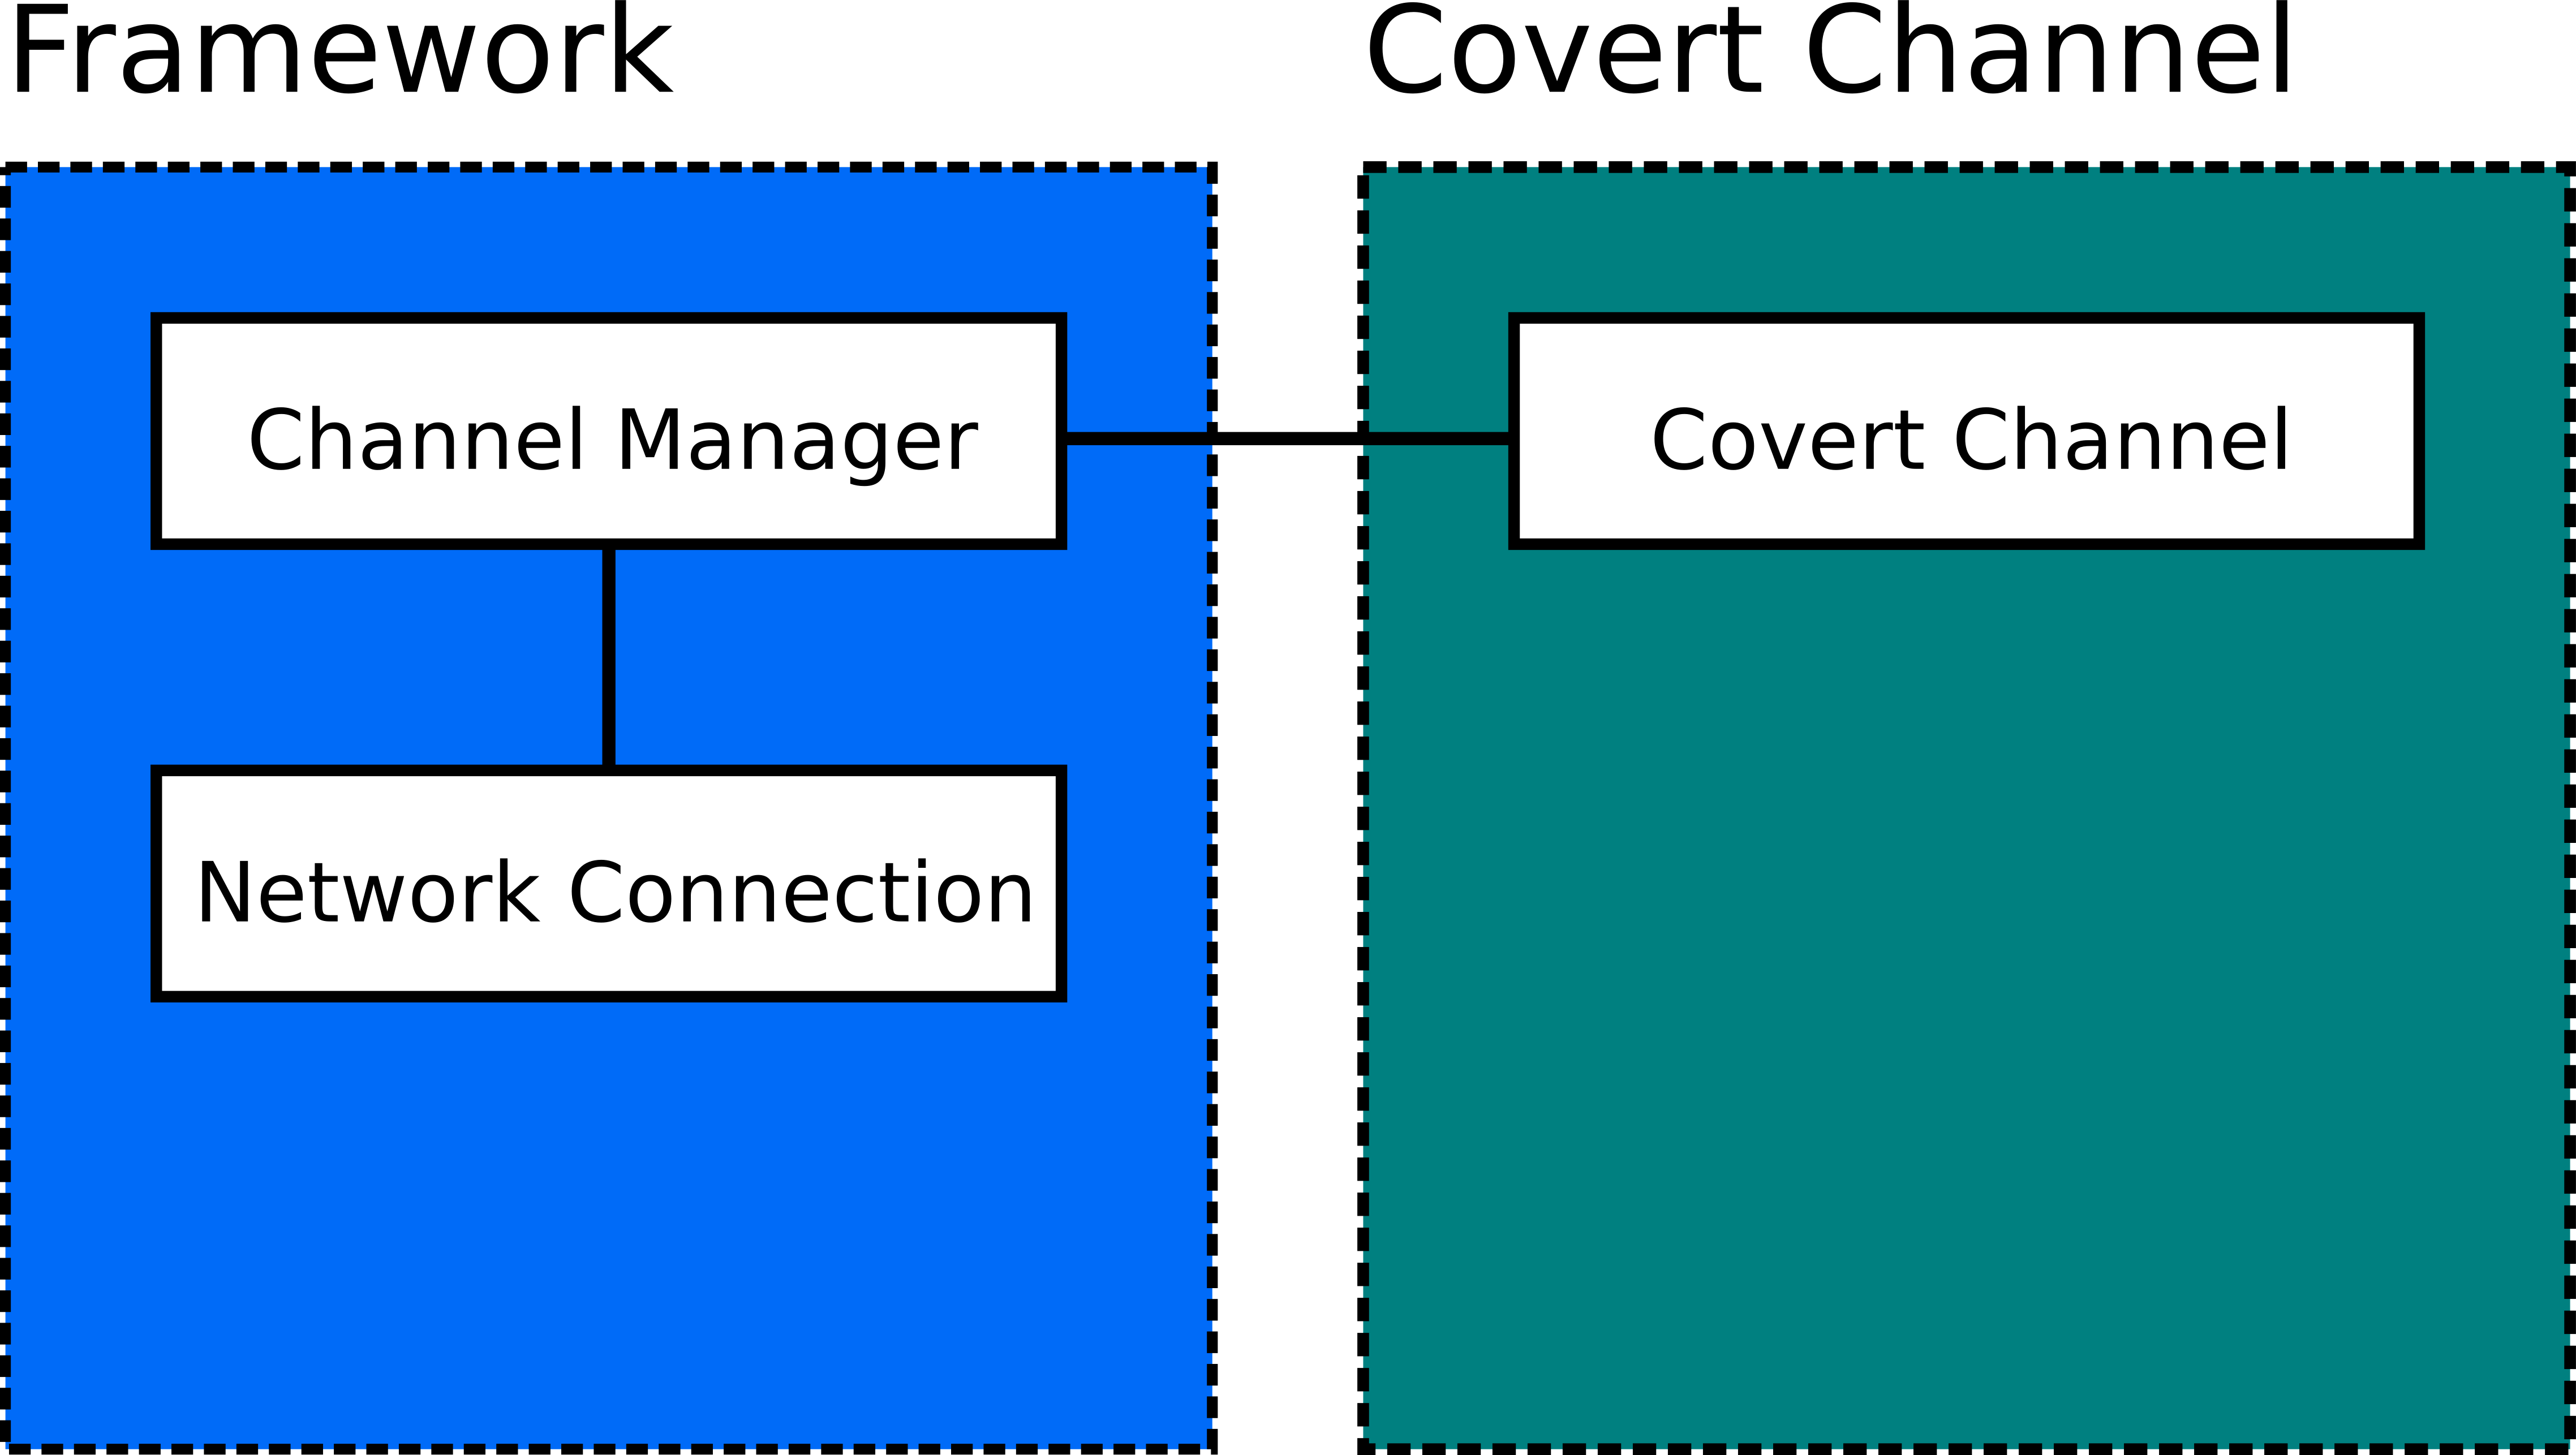
\includegraphics[scale=.4]{../Bilder/module.png}
		\end{figure}
\end{frame}

\begin{frame}

	\frametitle{QS-Ziele und ihre Sichherstellung}
\begin{center}
	\begin{itemize}
		\item \textbf{Zuverl�ssigkeit} \\
		{\begin{itemize}
			\item automatisierte Tests mit Boost.Test
			\item Ticket-System im SCM-Server
			\item Code Reviews
		\end{itemize}}
		\item \textbf{Testbarkeit}	\\
		{\begin{itemize}
			\item Zuteilung der Aufgaben an Module
			\item eigene Tests schreiben
			\item Architektur bei Problemen anpassen
		\end{itemize}}
	\end{itemize}
\end{center}

\end{frame}

\begin{frame}
	\frametitle{Zeitaufwand}
	\begin{center}
		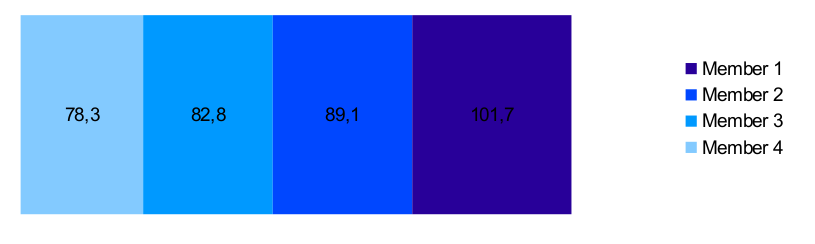
\includegraphics[scale=0.35]{../Bilder/memberStunden.png} \newline
	\end{center}

\end{frame}

\begin{frame}
\frametitle{Zeitmanagement}
		\begin{figure}
			\centering
			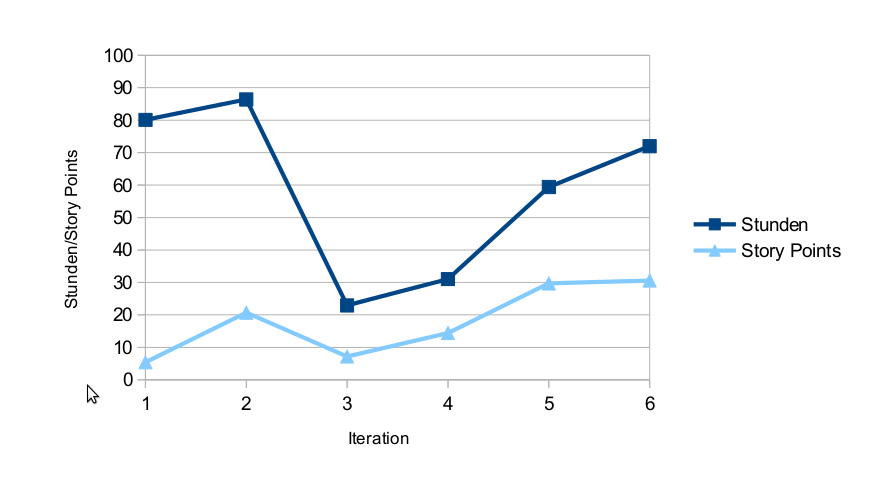
\includegraphics[scale=0.35]{../Bilder/stundenStoryPoints.png}
		\end{figure}
\end{frame}

\begin{frame}
\frametitle{Zeitmanagement}
		\begin{figure}
			\centering
			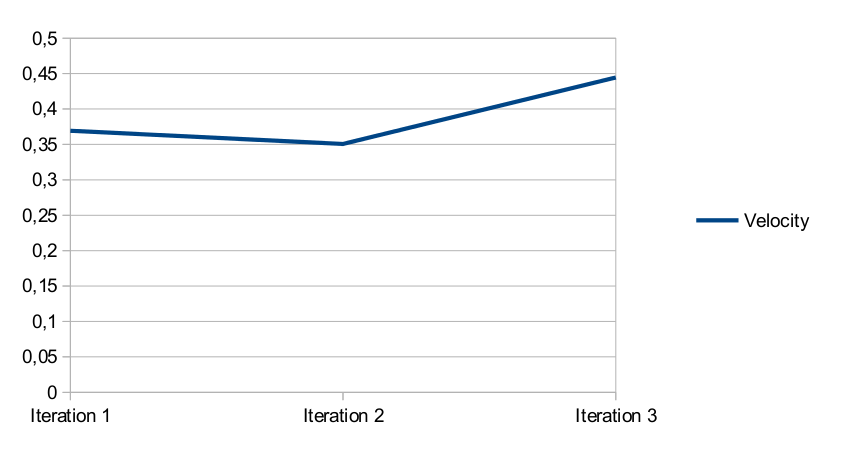
\includegraphics[scale=0.3]{../Bilder/velocity.png}
		\end{figure}
\end{frame}

\begin{frame}
\frametitle{Zusammenfassung}
	\vspace{.7cm}
	\hfill
	\begin{minipage}{.85\linewidth}
	\begin{itemize}
		\item Entwicklung einer modularen Bibliothek		
		\item Implementierung von Covert Channels zur versteckten Kommunikation
		\item Nutzbar f�r m�glichst viele Covert Channels
		\item Ver�ffentlichung als Open Source unter GPL Lizenz
		\item Nutzbar f�r verschiedene Anwender
	\end{itemize}
	\end{minipage}
\end{frame}


\end{document}